\documentclass[twoside]{book}

% Packages required by doxygen
\usepackage{fixltx2e}
\usepackage{calc}
\usepackage{doxygen}
\usepackage[export]{adjustbox} % also loads graphicx
\usepackage{graphicx}
\usepackage[utf8]{inputenc}
\usepackage{makeidx}
\usepackage{multicol}
\usepackage{multirow}
\PassOptionsToPackage{warn}{textcomp}
\usepackage{textcomp}
\usepackage[nointegrals]{wasysym}
\usepackage[table]{xcolor}

% Font selection
\usepackage[T1]{fontenc}
\usepackage[scaled=.90]{helvet}
\usepackage{courier}
\usepackage{amssymb}
\usepackage{sectsty}
\renewcommand{\familydefault}{\sfdefault}
\allsectionsfont{%
  \fontseries{bc}\selectfont%
  \color{darkgray}%
}
\renewcommand{\DoxyLabelFont}{%
  \fontseries{bc}\selectfont%
  \color{darkgray}%
}
\newcommand{\+}{\discretionary{\mbox{\scriptsize$\hookleftarrow$}}{}{}}

% Page & text layout
\usepackage{geometry}
\geometry{%
  a4paper,%
  top=2.5cm,%
  bottom=2.5cm,%
  left=2.5cm,%
  right=2.5cm%
}
\tolerance=750
\hfuzz=15pt
\hbadness=750
\setlength{\emergencystretch}{15pt}
\setlength{\parindent}{0cm}
\setlength{\parskip}{3ex plus 2ex minus 2ex}
\makeatletter
\renewcommand{\paragraph}{%
  \@startsection{paragraph}{4}{0ex}{-1.0ex}{1.0ex}{%
    \normalfont\normalsize\bfseries\SS@parafont%
  }%
}
\renewcommand{\subparagraph}{%
  \@startsection{subparagraph}{5}{0ex}{-1.0ex}{1.0ex}{%
    \normalfont\normalsize\bfseries\SS@subparafont%
  }%
}
\makeatother

% Headers & footers
\usepackage{fancyhdr}
\pagestyle{fancyplain}
\fancyhead[LE]{\fancyplain{}{\bfseries\thepage}}
\fancyhead[CE]{\fancyplain{}{}}
\fancyhead[RE]{\fancyplain{}{\bfseries\leftmark}}
\fancyhead[LO]{\fancyplain{}{\bfseries\rightmark}}
\fancyhead[CO]{\fancyplain{}{}}
\fancyhead[RO]{\fancyplain{}{\bfseries\thepage}}
\fancyfoot[LE]{\fancyplain{}{}}
\fancyfoot[CE]{\fancyplain{}{}}
\fancyfoot[RE]{\fancyplain{}{\bfseries\scriptsize Generated by Doxygen }}
\fancyfoot[LO]{\fancyplain{}{\bfseries\scriptsize Generated by Doxygen }}
\fancyfoot[CO]{\fancyplain{}{}}
\fancyfoot[RO]{\fancyplain{}{}}
\renewcommand{\footrulewidth}{0.4pt}
\renewcommand{\chaptermark}[1]{%
  \markboth{#1}{}%
}
\renewcommand{\sectionmark}[1]{%
  \markright{\thesection\ #1}%
}

% Indices & bibliography
\usepackage{natbib}
\usepackage[titles]{tocloft}
\setcounter{tocdepth}{3}
\setcounter{secnumdepth}{5}
\makeindex

% Hyperlinks (required, but should be loaded last)
\usepackage{ifpdf}
\ifpdf
  \usepackage[pdftex,pagebackref=true]{hyperref}
\else
  \usepackage[ps2pdf,pagebackref=true]{hyperref}
\fi
\hypersetup{%
  colorlinks=true,%
  linkcolor=blue,%
  citecolor=blue,%
  unicode%
}

% Custom commands
\newcommand{\clearemptydoublepage}{%
  \newpage{\pagestyle{empty}\cleardoublepage}%
}

\usepackage{caption}
\captionsetup{labelsep=space,justification=centering,font={bf},singlelinecheck=off,skip=4pt,position=top}

%===== C O N T E N T S =====

\begin{document}

% Titlepage & ToC
\hypersetup{pageanchor=false,
             bookmarksnumbered=true,
             pdfencoding=unicode
            }
\pagenumbering{alph}
\begin{titlepage}
\vspace*{7cm}
\begin{center}%
{\Large Faker-\/\+VN }\\
\vspace*{1cm}
{\large Generated by Doxygen 1.8.13}\\
\end{center}
\end{titlepage}
\clearemptydoublepage
\pagenumbering{roman}
\tableofcontents
\clearemptydoublepage
\pagenumbering{arabic}
\hypersetup{pageanchor=true}

%--- Begin generated contents ---
\chapter{Faker}
\label{md_README}
\Hypertarget{md_README}
Faker là một thư viện được sử dụng trong P\+H\+P-\/ cái mà chúng ta sử dụng để khởi tạo ra dữ liệu ảo. Bạn có thể tạo dữ liệu trực tiếp thông qua database console hay G\+UI hoặc một đoạn mã script php nào đó, có thể đáp ứng nhu cầu của bạn nhưng dữ liệu được tao ra lúc này có thể không giống thực tế lắm. Với thư viện Faker bạn có tạo ra dữ liệu giả nhưng không khác gì dữ liệu thật

\section*{Các nội dung chính}


\begin{DoxyItemize}
\item \href{#1}{\tt Cài Đặt}
\item \href{#export}{\tt Output}
\begin{DoxyItemize}
\item \href{#1}{\tt Name}
\end{DoxyItemize}
\end{DoxyItemize}

\subsection*{Cài Đặt}

Chúng ta có nhiều cách cài đặt nó, bạn có thể tải nó về song sau đó copy vào thư mục project của bạn, nhưng tôi khuyên bạn nên dùng composer cho công việc này, để cài đặt nó bạn chỉ cần chạy lệnh này trong project của bạn\+:

composer require nguyenthang0110/fakername1

$\ast$$\ast$ chú ý\+: Faker yêu cầu P\+HP bản 5.\+3 trở lên \subsection*{Cách sử dụng}

Do chúng ta cài Faker thông qua commposer nên để sử dụng nó bạn chỉ cần nạp tập tin autoload trong thư mục mà bạn muốn dùng \begin{DoxyVerb}require_once "vendor/autoload.php";
\end{DoxyVerb}


\subsection*{Sử dụng cơ bản}

Mọi thứ cấu hình coi như đã xong, việc kế tiếp là bạn khởi tạo một class của nó, chúng ta hãy xem xét ví dụ dưới đây\+: \begin{DoxyVerb}use Faker\Fake;
\end{DoxyVerb}


\subsubsection*{Create Fake Class (Example)}

\begin{DoxyVerb}$faker = Faker\Factory::create();
 //khoi tao đối tượng faker
echo $faker->name;
// Nguyễn Minh Nam
\end{DoxyVerb}


Nếu ví dụ này thể hiện các thuộc tính, chúng ta có thể gọi từng thuộc tính để in ra các kết quả khác nhau bởi vì các thuộc tính như name, address, phone được định nghĩa ngay trong class Fake, trong đó có các hàm \+\_\+\+\_\+contruct() để khởi tạo và hàm \+\_\+\+\_\+get() để trả về các giá trị \begin{DoxyVerb}<?php
for ($i = 0; $i < 5; $i++) {
echo $faker->name, "\n";
}
//Lê Văn Toàn
// Nguyễn Gia Long
//Phạm Thị Phương
//Lương Văn Thập
//Đặng Thị Oanh
\end{DoxyVerb}


Cụ thể Faker này cung cấp rất chi tiết, ở đây, nó cung cấp rất nhiều định dạng Ví dụ\+: \begin{DoxyVerb}titleMale                                 // 'Ông'
titleFemale                               // 'Bà'
firstNameMale                             // 'Trung'
lasttName                                 // 'Nguyễn'
middleNameMale or middleName('Male')      // 'Thi'
nameFemale                                // 'Phạm Thị Trang'
name('Male') or name('male')              //  'Nguyễn CHung Hiếu'
name('Female') or name('female')          // 'Lê Văn An'
\end{DoxyVerb}


\subsubsection*{Web html}

use Faker; \$fake=new Fake(); ?$>$ $<$?php for (\$i=0; \$i $<$ 10; \$i++)\+: ?$>$ \section*{$<$?php echo \$fake-\/$>$name ;?$>$}





$<$?php endfor; ?$>$

\subsubsection*{Tạo project sử dụng package này}

B1\+: tạo một thư mục rồi require package này về \+: composer require nguyenminhthang/faker

B2\+: tạo một file test ở ngay ngoài thư mục và test nội dung theo ý muốn

B3\+: sử dụng theo hướng dẫn\+: ví dụ tạo ra file in ra danh sách trúng thưởng số số Miền Bắc \begin{DoxyVerb}<?php
require __DIR__ . '/vendor/autoload.php';
$faker = Faker\Factory::create();
echo "Danh sách trúng sổ số Miền Bắc hôm nay"."\n";
echo "Giải Đặc Biệt : ". $faker->name('male'). "\n";
echo "Giải Nhất : ".$faker->name('male'). "\n";
echo "Giải Nhì : ".$faker->name('male'). "\n";
echo "Giải Ba : ".$faker->name('male'). "\n";
echo "Giải Khuyến Khích : ".$faker->name('male'). "\n";
\end{DoxyVerb}
 \subsubsection*{Thu được kết quả sau\+:}

Danh sách trúng sổ số Miền Bắc hôm nay Giải Đặc Biệt \+: Nghiêm Phượng Cẩn Giải Nhất \+: Trương Phương Án Giải Nhì \+: Lâm Như Trác Giải Ba \+: Xa Nhất Diệp Giải Khuyến Khích \+: Hình Khánh Đạo 
\chapter{Hierarchical Index}
\section{Class Hierarchy}
This inheritance list is sorted roughly, but not completely, alphabetically\+:\begin{DoxyCompactList}
\item \contentsline{section}{Faker\textbackslash{}Provider\textbackslash{}Base}{\pageref{classFaker_1_1Provider_1_1Base}}{}
\begin{DoxyCompactList}
\item \contentsline{section}{Faker\textbackslash{}Provider\textbackslash{}Person}{\pageref{classFaker_1_1Provider_1_1Person}}{}
\begin{DoxyCompactList}
\item \contentsline{section}{Faker\textbackslash{}Provider\textbackslash{}vi\+\_\+\+VN\textbackslash{}Person}{\pageref{classFaker_1_1Provider_1_1vi__VN_1_1Person}}{}
\end{DoxyCompactList}
\end{DoxyCompactList}
\item \contentsline{section}{Faker\textbackslash{}Factory}{\pageref{classFaker_1_1Factory}}{}
\item \contentsline{section}{Faker\textbackslash{}Generator}{\pageref{classFaker_1_1Generator}}{}
\end{DoxyCompactList}

\chapter{Class Index}
\section{Class List}
Here are the classes, structs, unions and interfaces with brief descriptions\+:\begin{DoxyCompactList}
\item\contentsline{section}{\hyperlink{classFaker_1_1Provider_1_1Base}{Faker\textbackslash{}\+Provider\textbackslash{}\+Base} }{\pageref{classFaker_1_1Provider_1_1Base}}{}
\item\contentsline{section}{\hyperlink{classFaker_1_1Factory}{Faker\textbackslash{}\+Factory} }{\pageref{classFaker_1_1Factory}}{}
\item\contentsline{section}{\hyperlink{classFaker_1_1Generator}{Faker\textbackslash{}\+Generator} }{\pageref{classFaker_1_1Generator}}{}
\item\contentsline{section}{\hyperlink{classFaker_1_1Provider_1_1vi__VN_1_1Person}{Faker\textbackslash{}\+Provider\textbackslash{}vi\+\_\+\+V\+N\textbackslash{}\+Person} }{\pageref{classFaker_1_1Provider_1_1vi__VN_1_1Person}}{}
\item\contentsline{section}{\hyperlink{classFaker_1_1Provider_1_1Person}{Faker\textbackslash{}\+Provider\textbackslash{}\+Person} }{\pageref{classFaker_1_1Provider_1_1Person}}{}
\end{DoxyCompactList}

\chapter{Class Documentation}
\hypertarget{classFaker_1_1Provider_1_1Base}{}\section{Faker\textbackslash{}Provider\textbackslash{}Base Class Reference}
\label{classFaker_1_1Provider_1_1Base}\index{Faker\textbackslash{}\+Provider\textbackslash{}\+Base@{Faker\textbackslash{}\+Provider\textbackslash{}\+Base}}


Inheritance diagram for Faker\textbackslash{}Provider\textbackslash{}Base\+:\nopagebreak
\begin{figure}[H]
\begin{center}
\leavevmode
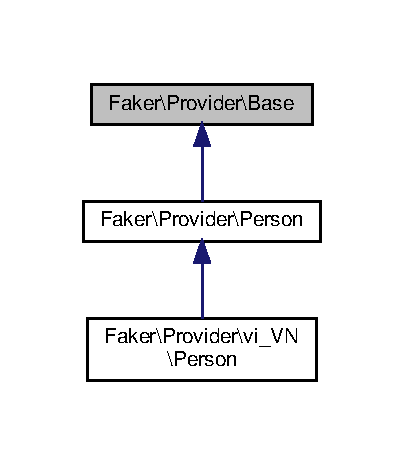
\includegraphics[width=194pt]{classFaker_1_1Provider_1_1Base__inherit__graph}
\end{center}
\end{figure}
\subsection*{Public Member Functions}
\begin{DoxyCompactItemize}
\item 
\mbox{\Hypertarget{classFaker_1_1Provider_1_1Base_a533c5296f9d9601d17fb9ad255d9fd5b}\label{classFaker_1_1Provider_1_1Base_a533c5296f9d9601d17fb9ad255d9fd5b}} 
{\bfseries \+\_\+\+\_\+construct} (\hyperlink{classFaker_1_1Generator}{Generator} \$generator)
\end{DoxyCompactItemize}
\subsection*{Protected Attributes}
\begin{DoxyCompactItemize}
\item 
\mbox{\Hypertarget{classFaker_1_1Provider_1_1Base_ad0b9e102a8a02c5ee52f26aaeafcd203}\label{classFaker_1_1Provider_1_1Base_ad0b9e102a8a02c5ee52f26aaeafcd203}} 
{\bfseries \$generator}
\end{DoxyCompactItemize}


The documentation for this class was generated from the following file\+:\begin{DoxyCompactItemize}
\item 
src/\+Faker/\+Provider/Base.\+php\end{DoxyCompactItemize}

\hypertarget{classFaker_1_1Factory}{}\section{Faker\textbackslash{}Factory Class Reference}
\label{classFaker_1_1Factory}\index{Faker\textbackslash{}\+Factory@{Faker\textbackslash{}\+Factory}}
\subsection*{Static Public Member Functions}
\begin{DoxyCompactItemize}
\item 
static \hyperlink{classFaker_1_1Factory_a98e6f274219744ee33c7434c1d2668ad}{create} (\$locale=self\+::\+D\+E\+F\+A\+U\+L\+T\+\_\+\+L\+O\+C\+A\+LE)
\end{DoxyCompactItemize}
\subsection*{Public Attributes}
\begin{DoxyCompactItemize}
\item 
\mbox{\Hypertarget{classFaker_1_1Factory_a2e6398cb8fab0e3296424a76bc982050}\label{classFaker_1_1Factory_a2e6398cb8fab0e3296424a76bc982050}} 
const {\bfseries D\+E\+F\+A\+U\+L\+T\+\_\+\+L\+O\+C\+A\+LE} = \textquotesingle{}vi\+\_\+\+VN\textquotesingle{}
\end{DoxyCompactItemize}
\subsection*{Static Protected Member Functions}
\begin{DoxyCompactItemize}
\item 
static \hyperlink{classFaker_1_1Factory_aa70262f20e04ea6091a61adc848c0631}{get\+Provider\+Classname} (\$provider, \$locale=\textquotesingle{}\textquotesingle{})
\begin{DoxyCompactList}\small\item\em thang dep trai 2 \end{DoxyCompactList}\item 
static \hyperlink{classFaker_1_1Factory_a775386565ba237a11fccd08f29fecfb7}{find\+Provider\+Classname} (\$provider, \$locale=\textquotesingle{}\textquotesingle{})
\end{DoxyCompactItemize}
\subsection*{Static Protected Attributes}
\begin{DoxyCompactItemize}
\item 
\mbox{\Hypertarget{classFaker_1_1Factory_ad397e0c679c72af873911350b2232187}\label{classFaker_1_1Factory_ad397e0c679c72af873911350b2232187}} 
static {\bfseries \$default\+Providers} = array( \textquotesingle{}Person\textquotesingle{})
\end{DoxyCompactItemize}


\subsection{Member Function Documentation}
\mbox{\Hypertarget{classFaker_1_1Factory_a98e6f274219744ee33c7434c1d2668ad}\label{classFaker_1_1Factory_a98e6f274219744ee33c7434c1d2668ad}} 
\index{Faker\+::\+Factory@{Faker\+::\+Factory}!create@{create}}
\index{create@{create}!Faker\+::\+Factory@{Faker\+::\+Factory}}
\subsubsection{\texorpdfstring{create()}{create()}}
{\footnotesize\ttfamily static Faker\textbackslash{}\+Factory\+::create (\begin{DoxyParamCaption}\item[{}]{\$locale = {\ttfamily self\+:\+:DEFAULT\+\_\+LOCALE} }\end{DoxyParamCaption})\hspace{0.3cm}{\ttfamily [static]}}

Create a new generator


\begin{DoxyParams}[1]{Parameters}
string & {\em \$locale} & \\
\hline
\end{DoxyParams}
\begin{DoxyReturn}{Returns}
\hyperlink{classFaker_1_1Generator}{Generator} 
\end{DoxyReturn}
\mbox{\Hypertarget{classFaker_1_1Factory_a775386565ba237a11fccd08f29fecfb7}\label{classFaker_1_1Factory_a775386565ba237a11fccd08f29fecfb7}} 
\index{Faker\+::\+Factory@{Faker\+::\+Factory}!find\+Provider\+Classname@{find\+Provider\+Classname}}
\index{find\+Provider\+Classname@{find\+Provider\+Classname}!Faker\+::\+Factory@{Faker\+::\+Factory}}
\subsubsection{\texorpdfstring{find\+Provider\+Classname()}{findProviderClassname()}}
{\footnotesize\ttfamily static Faker\textbackslash{}\+Factory\+::find\+Provider\+Classname (\begin{DoxyParamCaption}\item[{}]{\$provider,  }\item[{}]{\$locale = {\ttfamily \textquotesingle{}\textquotesingle{}} }\end{DoxyParamCaption})\hspace{0.3cm}{\ttfamily [static]}, {\ttfamily [protected]}}


\begin{DoxyParams}[1]{Parameters}
string & {\em \$provider} & \\
\hline
string & {\em \$locale} & \\
\hline
\end{DoxyParams}
\begin{DoxyReturn}{Returns}
string 
\end{DoxyReturn}
\mbox{\Hypertarget{classFaker_1_1Factory_aa70262f20e04ea6091a61adc848c0631}\label{classFaker_1_1Factory_aa70262f20e04ea6091a61adc848c0631}} 
\index{Faker\+::\+Factory@{Faker\+::\+Factory}!get\+Provider\+Classname@{get\+Provider\+Classname}}
\index{get\+Provider\+Classname@{get\+Provider\+Classname}!Faker\+::\+Factory@{Faker\+::\+Factory}}
\subsubsection{\texorpdfstring{get\+Provider\+Classname()}{getProviderClassname()}}
{\footnotesize\ttfamily static Faker\textbackslash{}\+Factory\+::get\+Provider\+Classname (\begin{DoxyParamCaption}\item[{}]{\$provider,  }\item[{}]{\$locale = {\ttfamily \textquotesingle{}\textquotesingle{}} }\end{DoxyParamCaption})\hspace{0.3cm}{\ttfamily [static]}, {\ttfamily [protected]}}



thang dep trai 2 


\begin{DoxyParams}[1]{Parameters}
string & {\em \$provider} & \\
\hline
string & {\em \$locale} & \\
\hline
\end{DoxyParams}
\begin{DoxyReturn}{Returns}
string thang dep trai 1 
\end{DoxyReturn}


The documentation for this class was generated from the following file\+:\begin{DoxyCompactItemize}
\item 
src/\+Faker/Factory.\+php\end{DoxyCompactItemize}

\hypertarget{classFaker_1_1Generator}{}\section{Faker\textbackslash{}Generator Class Reference}
\label{classFaker_1_1Generator}\index{Faker\textbackslash{}\+Generator@{Faker\textbackslash{}\+Generator}}
\subsection*{Public Member Functions}
\begin{DoxyCompactItemize}
\item 
\mbox{\Hypertarget{classFaker_1_1Generator_a7e6c5fd4053b6e78b9ca28dfbfab3966}\label{classFaker_1_1Generator_a7e6c5fd4053b6e78b9ca28dfbfab3966}} 
{\bfseries add\+Provider} (\$provider)
\item 
\mbox{\Hypertarget{classFaker_1_1Generator_a27e1507d90018984e40fa34f6b744a75}\label{classFaker_1_1Generator_a27e1507d90018984e40fa34f6b744a75}} 
{\bfseries get\+Providers} ()
\item 
\mbox{\Hypertarget{classFaker_1_1Generator_a79eb6bb6e45d4c10e73a8daecbedb30e}\label{classFaker_1_1Generator_a79eb6bb6e45d4c10e73a8daecbedb30e}} 
{\bfseries format} (\$formatter, \$arguments=array())
\item 
\hyperlink{classFaker_1_1Generator_a13fcdc32bea33cdc2a6befa9b4519de4}{get\+Formatter} (\$formatter)
\item 
\hyperlink{classFaker_1_1Generator_a546a92d05f70fe8716c5948a67fd276f}{parse} (\$string)
\item 
\hyperlink{classFaker_1_1Generator_aae756582311926f4d61ad376038fa85f}{\+\_\+\+\_\+get} (\$attribute)
\item 
\hyperlink{classFaker_1_1Generator_aa717daf0edbda2f413ab8dd1045a722e}{\+\_\+\+\_\+call} (\$method, \$attributes)
\end{DoxyCompactItemize}
\subsection*{Protected Member Functions}
\begin{DoxyCompactItemize}
\item 
\mbox{\Hypertarget{classFaker_1_1Generator_afbde496805f567bfc58f00753fe3b8bb}\label{classFaker_1_1Generator_afbde496805f567bfc58f00753fe3b8bb}} 
{\bfseries call\+Format\+With\+Matches} (\$matches)
\end{DoxyCompactItemize}
\subsection*{Protected Attributes}
\begin{DoxyCompactItemize}
\item 
\mbox{\Hypertarget{classFaker_1_1Generator_a0129c2f5d5a9f0ec56ffa2f34f8c441b}\label{classFaker_1_1Generator_a0129c2f5d5a9f0ec56ffa2f34f8c441b}} 
{\bfseries \$providers} = array()
\item 
\mbox{\Hypertarget{classFaker_1_1Generator_acc25fb560a2732d22ca081ac414e5907}\label{classFaker_1_1Generator_acc25fb560a2732d22ca081ac414e5907}} 
{\bfseries \$formatters} = array()
\end{DoxyCompactItemize}


\subsection{Member Function Documentation}
\mbox{\Hypertarget{classFaker_1_1Generator_aa717daf0edbda2f413ab8dd1045a722e}\label{classFaker_1_1Generator_aa717daf0edbda2f413ab8dd1045a722e}} 
\index{Faker\+::\+Generator@{Faker\+::\+Generator}!\+\_\+\+\_\+call@{\+\_\+\+\_\+call}}
\index{\+\_\+\+\_\+call@{\+\_\+\+\_\+call}!Faker\+::\+Generator@{Faker\+::\+Generator}}
\subsubsection{\texorpdfstring{\+\_\+\+\_\+call()}{\_\_call()}}
{\footnotesize\ttfamily Faker\textbackslash{}\+Generator\+::\+\_\+\+\_\+call (\begin{DoxyParamCaption}\item[{}]{\$method,  }\item[{}]{\$attributes }\end{DoxyParamCaption})}


\begin{DoxyParams}[1]{Parameters}
string & {\em \$method} & \\
\hline
array & {\em \$attributes} & \\
\hline
\end{DoxyParams}
\begin{DoxyReturn}{Returns}
mixed 
\end{DoxyReturn}
\mbox{\Hypertarget{classFaker_1_1Generator_aae756582311926f4d61ad376038fa85f}\label{classFaker_1_1Generator_aae756582311926f4d61ad376038fa85f}} 
\index{Faker\+::\+Generator@{Faker\+::\+Generator}!\+\_\+\+\_\+get@{\+\_\+\+\_\+get}}
\index{\+\_\+\+\_\+get@{\+\_\+\+\_\+get}!Faker\+::\+Generator@{Faker\+::\+Generator}}
\subsubsection{\texorpdfstring{\+\_\+\+\_\+get()}{\_\_get()}}
{\footnotesize\ttfamily Faker\textbackslash{}\+Generator\+::\+\_\+\+\_\+get (\begin{DoxyParamCaption}\item[{}]{\$attribute }\end{DoxyParamCaption})}


\begin{DoxyParams}[1]{Parameters}
string & {\em \$attribute} & \\
\hline
\end{DoxyParams}
\begin{DoxyReturn}{Returns}
mixed 
\end{DoxyReturn}
\mbox{\Hypertarget{classFaker_1_1Generator_a13fcdc32bea33cdc2a6befa9b4519de4}\label{classFaker_1_1Generator_a13fcdc32bea33cdc2a6befa9b4519de4}} 
\index{Faker\+::\+Generator@{Faker\+::\+Generator}!get\+Formatter@{get\+Formatter}}
\index{get\+Formatter@{get\+Formatter}!Faker\+::\+Generator@{Faker\+::\+Generator}}
\subsubsection{\texorpdfstring{get\+Formatter()}{getFormatter()}}
{\footnotesize\ttfamily Faker\textbackslash{}\+Generator\+::get\+Formatter (\begin{DoxyParamCaption}\item[{}]{\$formatter }\end{DoxyParamCaption})}


\begin{DoxyParams}[1]{Parameters}
string & {\em \$formatter} & \\
\hline
\end{DoxyParams}
\begin{DoxyReturn}{Returns}
Callable 
\end{DoxyReturn}
\mbox{\Hypertarget{classFaker_1_1Generator_a546a92d05f70fe8716c5948a67fd276f}\label{classFaker_1_1Generator_a546a92d05f70fe8716c5948a67fd276f}} 
\index{Faker\+::\+Generator@{Faker\+::\+Generator}!parse@{parse}}
\index{parse@{parse}!Faker\+::\+Generator@{Faker\+::\+Generator}}
\subsubsection{\texorpdfstring{parse()}{parse()}}
{\footnotesize\ttfamily Faker\textbackslash{}\+Generator\+::parse (\begin{DoxyParamCaption}\item[{}]{\$string }\end{DoxyParamCaption})}

Replaces tokens (\textquotesingle{}\{\{ token\+Name \}\}\textquotesingle{}) with the result from the token method call


\begin{DoxyParams}[1]{Parameters}
string & {\em \$string} & String that needs to bet parsed \\
\hline
\end{DoxyParams}
\begin{DoxyReturn}{Returns}
string 
\end{DoxyReturn}


The documentation for this class was generated from the following file\+:\begin{DoxyCompactItemize}
\item 
src/\+Faker/Generator.\+php\end{DoxyCompactItemize}

\hypertarget{classFaker_1_1Provider_1_1vi__VN_1_1Person}{}\section{Faker\textbackslash{}Provider\textbackslash{}vi\+\_\+\+VN\textbackslash{}Person Class Reference}
\label{classFaker_1_1Provider_1_1vi__VN_1_1Person}\index{Faker\textbackslash{}\+Provider\textbackslash{}vi\+\_\+\+V\+N\textbackslash{}\+Person@{Faker\textbackslash{}\+Provider\textbackslash{}vi\+\_\+\+V\+N\textbackslash{}\+Person}}


Inheritance diagram for Faker\textbackslash{}Provider\textbackslash{}vi\+\_\+\+VN\textbackslash{}Person\+:\nopagebreak
\begin{figure}[H]
\begin{center}
\leavevmode
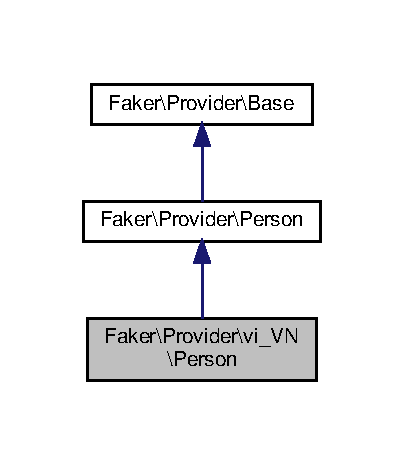
\includegraphics[width=194pt]{classFaker_1_1Provider_1_1vi__VN_1_1Person__inherit__graph}
\end{center}
\end{figure}


Collaboration diagram for Faker\textbackslash{}Provider\textbackslash{}vi\+\_\+\+VN\textbackslash{}Person\+:\nopagebreak
\begin{figure}[H]
\begin{center}
\leavevmode
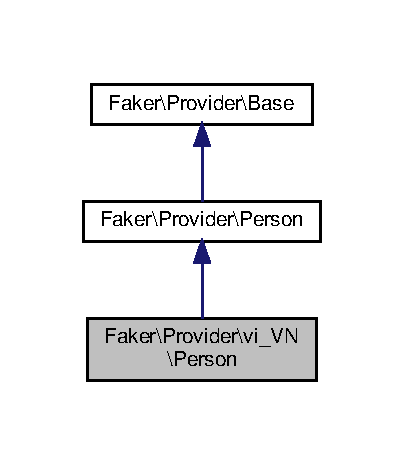
\includegraphics[width=194pt]{classFaker_1_1Provider_1_1vi__VN_1_1Person__coll__graph}
\end{center}
\end{figure}
\subsection*{Public Member Functions}
\begin{DoxyCompactItemize}
\item 
\mbox{\Hypertarget{classFaker_1_1Provider_1_1vi__VN_1_1Person_a33f7b77f00d3a4e5577fe46c90f09570}\label{classFaker_1_1Provider_1_1vi__VN_1_1Person_a33f7b77f00d3a4e5577fe46c90f09570}} 
{\bfseries middle\+Name} (\$gender=null)
\end{DoxyCompactItemize}
\subsection*{Static Public Member Functions}
\begin{DoxyCompactItemize}
\item 
\mbox{\Hypertarget{classFaker_1_1Provider_1_1vi__VN_1_1Person_ad5964a9b2fa71f244c187830b06f9503}\label{classFaker_1_1Provider_1_1vi__VN_1_1Person_ad5964a9b2fa71f244c187830b06f9503}} 
static {\bfseries middle\+Name\+Male} ()
\item 
\mbox{\Hypertarget{classFaker_1_1Provider_1_1vi__VN_1_1Person_abdd9185984d14569ac94d09bb6652544}\label{classFaker_1_1Provider_1_1vi__VN_1_1Person_abdd9185984d14569ac94d09bb6652544}} 
static {\bfseries middle\+Name\+Female} ()
\end{DoxyCompactItemize}
\subsection*{Static Protected Attributes}
\begin{DoxyCompactItemize}
\item 
static {\bfseries \$male\+Name\+Formats}
\item 
static {\bfseries \$female\+Name\+Formats}
\item 
static {\bfseries \$middle\+Name\+Format}
\item 
static \hyperlink{classFaker_1_1Provider_1_1vi__VN_1_1Person_a995e9705e8dca9f652bb254e4feed494}{\$first\+Name\+Male}
\item 
static \hyperlink{classFaker_1_1Provider_1_1vi__VN_1_1Person_acd4131a86a3ac6d21b0861fc0d2a19fc}{\$middle\+Name\+Male}
\item 
static \hyperlink{classFaker_1_1Provider_1_1vi__VN_1_1Person_aa5ac9daadabf51ad95df378b7e1d96b7}{\$first\+Name\+Female}
\item 
static \hyperlink{classFaker_1_1Provider_1_1vi__VN_1_1Person_ae9aca3674140ead2e5b8516259bf69e0}{\$middle\+Name\+Female}
\item 
static \hyperlink{classFaker_1_1Provider_1_1vi__VN_1_1Person_ad101126d2ae05f5991b82eee629f054a}{\$last\+Name}
\item 
\mbox{\Hypertarget{classFaker_1_1Provider_1_1vi__VN_1_1Person_a5b975f36cf21488876e4a06f7ab70707}\label{classFaker_1_1Provider_1_1vi__VN_1_1Person_a5b975f36cf21488876e4a06f7ab70707}} 
static {\bfseries \$title\+Male} = array(\textquotesingle{}Cụ\textquotesingle{}, \textquotesingle{}Ông\textquotesingle{}, \textquotesingle{}Bác\textquotesingle{}, \textquotesingle{}Chú\textquotesingle{}, \textquotesingle{}Anh\textquotesingle{}, \textquotesingle{}Em\textquotesingle{})
\item 
\mbox{\Hypertarget{classFaker_1_1Provider_1_1vi__VN_1_1Person_a530ff3c2fe73a11f286a9565574149c6}\label{classFaker_1_1Provider_1_1vi__VN_1_1Person_a530ff3c2fe73a11f286a9565574149c6}} 
static {\bfseries \$title\+Female} = array(\textquotesingle{}Cụ\textquotesingle{}, \textquotesingle{}Bà\textquotesingle{}, \textquotesingle{}Bác\textquotesingle{}, \textquotesingle{}Cô\textquotesingle{}, \textquotesingle{}Chị\textquotesingle{}, \textquotesingle{}Em\textquotesingle{})
\end{DoxyCompactItemize}
\subsection*{Additional Inherited Members}


\subsection{Member Data Documentation}
\mbox{\Hypertarget{classFaker_1_1Provider_1_1vi__VN_1_1Person_a87cff5ca95ab1608efbd06ab55239018}\label{classFaker_1_1Provider_1_1vi__VN_1_1Person_a87cff5ca95ab1608efbd06ab55239018}} 
\index{Faker\+::\+Provider\+::vi\+\_\+\+V\+N\+::\+Person@{Faker\+::\+Provider\+::vi\+\_\+\+V\+N\+::\+Person}!\$female\+Name\+Formats@{\$female\+Name\+Formats}}
\index{\$female\+Name\+Formats@{\$female\+Name\+Formats}!Faker\+::\+Provider\+::vi\+\_\+\+V\+N\+::\+Person@{Faker\+::\+Provider\+::vi\+\_\+\+V\+N\+::\+Person}}
\subsubsection{\texorpdfstring{\$female\+Name\+Formats}{$femaleNameFormats}}
{\footnotesize\ttfamily Faker\textbackslash{}\+Provider\textbackslash{}vi\+\_\+\+V\+N\textbackslash{}\+Person\+::\$female\+Name\+Formats\hspace{0.3cm}{\ttfamily [static]}, {\ttfamily [protected]}}

{\bfseries Initial value\+:}
\begin{DoxyCode}
= array(

        \textcolor{stringliteral}{'\{\{lastName\}\} \{\{middleNameFemale\}\} \{\{firstNameFemale\}\}'},
       
    )
\end{DoxyCode}
\mbox{\Hypertarget{classFaker_1_1Provider_1_1vi__VN_1_1Person_aa5ac9daadabf51ad95df378b7e1d96b7}\label{classFaker_1_1Provider_1_1vi__VN_1_1Person_aa5ac9daadabf51ad95df378b7e1d96b7}} 
\index{Faker\+::\+Provider\+::vi\+\_\+\+V\+N\+::\+Person@{Faker\+::\+Provider\+::vi\+\_\+\+V\+N\+::\+Person}!\$first\+Name\+Female@{\$first\+Name\+Female}}
\index{\$first\+Name\+Female@{\$first\+Name\+Female}!Faker\+::\+Provider\+::vi\+\_\+\+V\+N\+::\+Person@{Faker\+::\+Provider\+::vi\+\_\+\+V\+N\+::\+Person}}
\subsubsection{\texorpdfstring{\$first\+Name\+Female}{$firstNameFemale}}
{\footnotesize\ttfamily Faker\textbackslash{}\+Provider\textbackslash{}vi\+\_\+\+V\+N\textbackslash{}\+Person\+::\$first\+Name\+Female\hspace{0.3cm}{\ttfamily [static]}, {\ttfamily [protected]}}

{\bfseries Initial value\+:}
\begin{DoxyCode}
= array(
        \textcolor{stringliteral}{'An'}, \textcolor{stringliteral}{'Anh'},
        \textcolor{stringliteral}{'Bình'}, \textcolor{stringliteral}{'Bích'}, \textcolor{stringliteral}{'Băng'}, \textcolor{stringliteral}{'Bạch'}, \textcolor{stringliteral}{'Bảo'},
        \textcolor{stringliteral}{'Ca'}, \textcolor{stringliteral}{'Chi'}, \textcolor{stringliteral}{'Chinh'}, \textcolor{stringliteral}{'Chiêu'}, \textcolor{stringliteral}{'Chung'}, \textcolor{stringliteral}{'Châu'}, \textcolor{stringliteral}{'Cát'}, \textcolor{stringliteral}{'Cúc'}, \textcolor{stringliteral}{'Cương'}, \textcolor{stringliteral}{'Cầm'},
        \textcolor{stringliteral}{'Dao'}, \textcolor{stringliteral}{'Di'}, \textcolor{stringliteral}{'Diễm'}, \textcolor{stringliteral}{'Diệp'}, \textcolor{stringliteral}{'Diệu'}, \textcolor{stringliteral}{'Du'}, \textcolor{stringliteral}{'Dung'}, \textcolor{stringliteral}{'Duyên'}, \textcolor{stringliteral}{'Dân'}, \textcolor{stringliteral}{'Dương'},
        \textcolor{stringliteral}{'Giang'}, \textcolor{stringliteral}{'Giao'},
        \textcolor{stringliteral}{'Hiếu'}, \textcolor{stringliteral}{'Hiền'}, \textcolor{stringliteral}{'Hiệp'}, \textcolor{stringliteral}{'Hoa'}, \textcolor{stringliteral}{'Hoan'}, \textcolor{stringliteral}{'Hoài'}, \textcolor{stringliteral}{'Hoàn'}, \textcolor{stringliteral}{'Huyền'}, \textcolor{stringliteral}{'Huệ'}, \textcolor{stringliteral}{'Hà'}, \textcolor{stringliteral}{'Hân'}, \textcolor{stringliteral}{'Hòa'}, \textcolor{stringliteral}{'Hương'},
       \textcolor{stringliteral}{'Hường'}, \textcolor{stringliteral}{'Hạ'}, \textcolor{stringliteral}{'Hạnh'}, \textcolor{stringliteral}{'Hải'}, \textcolor{stringliteral}{'Hảo'}, \textcolor{stringliteral}{'Hậu'}, \textcolor{stringliteral}{'Hằng'}, \textcolor{stringliteral}{'Hồng'}, \textcolor{stringliteral}{'Hợp'},
        \textcolor{stringliteral}{'Khai'}, \textcolor{stringliteral}{'Khanh'}, \textcolor{stringliteral}{'Khuyên'}, \textcolor{stringliteral}{'Khuê'}, \textcolor{stringliteral}{'Khánh'}, \textcolor{stringliteral}{'Khê'}, \textcolor{stringliteral}{'Khôi'}, \textcolor{stringliteral}{'Kim'}, \textcolor{stringliteral}{'Kiều'},
        \textcolor{stringliteral}{'Lam'}, \textcolor{stringliteral}{'Lan'}, \textcolor{stringliteral}{'Linh'}, \textcolor{stringliteral}{'Liên'}, \textcolor{stringliteral}{'Liễu'}, \textcolor{stringliteral}{'Loan'}, \textcolor{stringliteral}{'Ly'}, \textcolor{stringliteral}{'Lâm'}, \textcolor{stringliteral}{'Lý'}, \textcolor{stringliteral}{'Lễ'}, \textcolor{stringliteral}{'Lệ'}, \textcolor{stringliteral}{'Lộc'}, \textcolor{stringliteral}{'Lợi'},
        \textcolor{stringliteral}{'Mai'}, \textcolor{stringliteral}{'Mi'}, \textcolor{stringliteral}{'Minh'}, \textcolor{stringliteral}{'Miên'}, \textcolor{stringliteral}{'My'}, \textcolor{stringliteral}{'Mẫn'}, \textcolor{stringliteral}{'Mỹ'},
        \textcolor{stringliteral}{'Nga'}, \textcolor{stringliteral}{'Nghi'}, \textcolor{stringliteral}{'Nguyên'}, \textcolor{stringliteral}{'Nguyệt'}, \textcolor{stringliteral}{'Ngà'}, \textcolor{stringliteral}{'Ngân'}, \textcolor{stringliteral}{'Ngôn'}, \textcolor{stringliteral}{'Ngọc'}, \textcolor{stringliteral}{'Nhi'}, \textcolor{stringliteral}{'Nhiên'}, \textcolor{stringliteral}{'Nhung'}, \textcolor{stringliteral}{'Nhàn'}, \textcolor{stringliteral}{
      'Nhân'}, \textcolor{stringliteral}{'Nhã'}, \textcolor{stringliteral}{'Như'}, \textcolor{stringliteral}{'Nương'}, \textcolor{stringliteral}{'Nữ'},
        \textcolor{stringliteral}{'Oanh'},
        \textcolor{stringliteral}{'Phi'},
        \textcolor{stringliteral}{'Phong'}, \textcolor{stringliteral}{'Phúc'}, \textcolor{stringliteral}{'Phương'}, \textcolor{stringliteral}{'Phước'}, \textcolor{stringliteral}{'Phượng'}, \textcolor{stringliteral}{'Phụng'},
        \textcolor{stringliteral}{'Quyên'}, \textcolor{stringliteral}{'Quân'}, \textcolor{stringliteral}{'Quế'}, \textcolor{stringliteral}{'Quỳnh'},
        \textcolor{stringliteral}{'Sa'}, \textcolor{stringliteral}{'San'}, \textcolor{stringliteral}{'Sinh'}, \textcolor{stringliteral}{'Sương'},
        \textcolor{stringliteral}{'Thanh'}, \textcolor{stringliteral}{'Thảo'}, \textcolor{stringliteral}{'Thi'}, \textcolor{stringliteral}{'Thiên'}, \textcolor{stringliteral}{'Thiện'}, \textcolor{stringliteral}{'Thoa'}, \textcolor{stringliteral}{'Thoại'}, \textcolor{stringliteral}{'Thu'}, \textcolor{stringliteral}{'Thuần'}, \textcolor{stringliteral}{'Thuận'}, \textcolor{stringliteral}{'Thy'}, \textcolor{stringliteral}{'Thêu'}, \textcolor{stringliteral}{
      'Thùy'}, \textcolor{stringliteral}{'Thúy'}, \textcolor{stringliteral}{'Thơ'}, \textcolor{stringliteral}{'Thư'}, \textcolor{stringliteral}{'Thương'}, \textcolor{stringliteral}{'Thường'}, \textcolor{stringliteral}{'Thảo'}, \textcolor{stringliteral}{'Thắm'}, \textcolor{stringliteral}{'Thục'}, \textcolor{stringliteral}{'Thủy'}, \textcolor{stringliteral}{'Tiên'}, \textcolor{stringliteral}{'Trang'}, \textcolor{stringliteral}{'Trinh'}, \textcolor{stringliteral}{
      'Trung'}, \textcolor{stringliteral}{'Trà'}, \textcolor{stringliteral}{'Trâm'}, \textcolor{stringliteral}{'Trân'}, \textcolor{stringliteral}{'Trúc'}, \textcolor{stringliteral}{'Trầm'}, \textcolor{stringliteral}{'Tuyến'}, \textcolor{stringliteral}{'Tuyết'}, \textcolor{stringliteral}{'Tuyền'}, \textcolor{stringliteral}{'Tuệ'}, \textcolor{stringliteral}{'Ty'}, \textcolor{stringliteral}{'Tâm'}, \textcolor{stringliteral}{'Tú'},
        \textcolor{stringliteral}{'Uyên'}, \textcolor{stringliteral}{'Uyển'},
        \textcolor{stringliteral}{'Vi'}, \textcolor{stringliteral}{'Việt'},
        \textcolor{stringliteral}{'Vy'}, \textcolor{stringliteral}{'Vân'}, \textcolor{stringliteral}{'Vũ'}, \textcolor{stringliteral}{'Vọng'}, \textcolor{stringliteral}{'Vỹ'},
        \textcolor{stringliteral}{'Xuyến'}, \textcolor{stringliteral}{'Xuân'},
        \textcolor{stringliteral}{'Yên'}, \textcolor{stringliteral}{'Yến'},
        \textcolor{stringliteral}{'Ái'}, \textcolor{stringliteral}{'Ánh'}, \textcolor{stringliteral}{'Ân'},
        \textcolor{stringliteral}{'Đan'}, \textcolor{stringliteral}{'Điệp'}, \textcolor{stringliteral}{'Đoan'}, \textcolor{stringliteral}{'Đài'}, \textcolor{stringliteral}{'Đàn'}, \textcolor{stringliteral}{'Đào'}, \textcolor{stringliteral}{'Đình'}, \textcolor{stringliteral}{'Đường'}, \textcolor{stringliteral}{'Đan'},
        \textcolor{stringliteral}{'Ý'},
    )
\end{DoxyCode}
\hyperlink{}{http\+://www.\+dattenhay.\+vn/1001-\/ten-\/cho-\/be-\/gai.\+htm}\mbox{\Hypertarget{classFaker_1_1Provider_1_1vi__VN_1_1Person_a995e9705e8dca9f652bb254e4feed494}\label{classFaker_1_1Provider_1_1vi__VN_1_1Person_a995e9705e8dca9f652bb254e4feed494}} 
\index{Faker\+::\+Provider\+::vi\+\_\+\+V\+N\+::\+Person@{Faker\+::\+Provider\+::vi\+\_\+\+V\+N\+::\+Person}!\$first\+Name\+Male@{\$first\+Name\+Male}}
\index{\$first\+Name\+Male@{\$first\+Name\+Male}!Faker\+::\+Provider\+::vi\+\_\+\+V\+N\+::\+Person@{Faker\+::\+Provider\+::vi\+\_\+\+V\+N\+::\+Person}}
\subsubsection{\texorpdfstring{\$first\+Name\+Male}{$firstNameMale}}
{\footnotesize\ttfamily Faker\textbackslash{}\+Provider\textbackslash{}vi\+\_\+\+V\+N\textbackslash{}\+Person\+::\$first\+Name\+Male\hspace{0.3cm}{\ttfamily [static]}, {\ttfamily [protected]}}

{\bfseries Initial value\+:}
\begin{DoxyCode}
= array(
        \textcolor{stringliteral}{'An'}, \textcolor{stringliteral}{'Anh'},
        \textcolor{stringliteral}{'Bào'}, \textcolor{stringliteral}{'Bình'}, \textcolor{stringliteral}{'Bạch'}, \textcolor{stringliteral}{'Bảo'}, \textcolor{stringliteral}{'Bắc'}, \textcolor{stringliteral}{'Bằng'}, \textcolor{stringliteral}{'Bổng'}, \textcolor{stringliteral}{'Bửu'},
        \textcolor{stringliteral}{'Ca'}, \textcolor{stringliteral}{'Canh'}, \textcolor{stringliteral}{'Chiến'}, \textcolor{stringliteral}{'Chiểu'}, \textcolor{stringliteral}{'Châu'}, \textcolor{stringliteral}{'Chính'}, \textcolor{stringliteral}{'Chương'}, \textcolor{stringliteral}{'Chưởng'}, \textcolor{stringliteral}{'Chấn'}, \textcolor{stringliteral}{'Công'}, \textcolor{stringliteral}{'Cơ'}, \textcolor{stringliteral}{'Cương'},
       \textcolor{stringliteral}{'Cường'}, \textcolor{stringliteral}{'Cảnh'}, \textcolor{stringliteral}{'Cần'}, \textcolor{stringliteral}{'Cẩn'},
        \textcolor{stringliteral}{'Danh'}, \textcolor{stringliteral}{'Di'}, \textcolor{stringliteral}{'Dinh'}, \textcolor{stringliteral}{'Diệp'}, \textcolor{stringliteral}{'Diệu'}, \textcolor{stringliteral}{'Du'}, \textcolor{stringliteral}{'Duy'}, \textcolor{stringliteral}{'Duệ'}, \textcolor{stringliteral}{'Dân'}, \textcolor{stringliteral}{'Dũng'}, \textcolor{stringliteral}{'Dương'}, \textcolor{stringliteral}{'Dụng'},
        \textcolor{stringliteral}{'Giang'}, \textcolor{stringliteral}{'Giác'}, \textcolor{stringliteral}{'Giáp'},
        \textcolor{stringliteral}{'Hiên'}, \textcolor{stringliteral}{'Hiếu'}, \textcolor{stringliteral}{'Hiền'}, \textcolor{stringliteral}{'Hiển'}, \textcolor{stringliteral}{'Hiệp'}, \textcolor{stringliteral}{'Hoa'}, \textcolor{stringliteral}{'Hoài'}, \textcolor{stringliteral}{'Hoàn'}, \textcolor{stringliteral}{'Hoàng'}, \textcolor{stringliteral}{'Hoán'}, \textcolor{stringliteral}{'Huy'}, \textcolor{stringliteral}{'Huynh'}, \textcolor{stringliteral}{'
      Huấn'}, \textcolor{stringliteral}{'Huỳnh'}, \textcolor{stringliteral}{'Hà'}, \textcolor{stringliteral}{'Hành'}, \textcolor{stringliteral}{'Hào'}, \textcolor{stringliteral}{'Hòa'}, \textcolor{stringliteral}{'Hùng'}, \textcolor{stringliteral}{'Hưng'}, \textcolor{stringliteral}{'Hạnh'}, \textcolor{stringliteral}{'Hải'}, \textcolor{stringliteral}{'Hảo'}, \textcolor{stringliteral}{'Hậu'}, \textcolor{stringliteral}{'Học'}, \textcolor{stringliteral}{'Hồng'}, \textcolor{stringliteral}{'Hội'},
       \textcolor{stringliteral}{'Hợp'}, \textcolor{stringliteral}{'Hữu'}, \textcolor{stringliteral}{'Hỷ'},
        \textcolor{stringliteral}{'Kha'}, \textcolor{stringliteral}{'Khang'}, \textcolor{stringliteral}{'Khanh'}, \textcolor{stringliteral}{'Khiêm'}, \textcolor{stringliteral}{'Khiếu'}, \textcolor{stringliteral}{'Khoa'}, \textcolor{stringliteral}{'Khoát'}, \textcolor{stringliteral}{'Khánh'}, \textcolor{stringliteral}{'Khôi'}, \textcolor{stringliteral}{'Khương'}, \textcolor{stringliteral}{'Khải'}, \textcolor{stringliteral}{'Kim
      '}, \textcolor{stringliteral}{'Kiên'}, \textcolor{stringliteral}{'Kiếm'}, \textcolor{stringliteral}{'Kiện'}, \textcolor{stringliteral}{'Kiệt'}, \textcolor{stringliteral}{'Kính'}, \textcolor{stringliteral}{'Kỳ'}, \textcolor{stringliteral}{'Kỷ'},
        \textcolor{stringliteral}{'Lai'}, \textcolor{stringliteral}{'Lam'}, \textcolor{stringliteral}{'Linh'}, \textcolor{stringliteral}{'Liêm'}, \textcolor{stringliteral}{'Long'}, \textcolor{stringliteral}{'Luận'}, \textcolor{stringliteral}{'Luật'}, \textcolor{stringliteral}{'Lâm'}, \textcolor{stringliteral}{'Lân'}, \textcolor{stringliteral}{'Lý'}, \textcolor{stringliteral}{'Lĩnh'}, \textcolor{stringliteral}{'Lương'}, \textcolor{stringliteral}{'Lạc'}, \textcolor{stringliteral}{'
      Lập'}, \textcolor{stringliteral}{'Lễ'}, \textcolor{stringliteral}{'Lộ'}, \textcolor{stringliteral}{'Lộc'}, \textcolor{stringliteral}{'Lực'},
        \textcolor{stringliteral}{'Minh'}, \textcolor{stringliteral}{'Mạnh'}, \textcolor{stringliteral}{'Mẫn'}, \textcolor{stringliteral}{'Mỹ'},
        \textcolor{stringliteral}{'Nam'}, \textcolor{stringliteral}{'Nghiêm'}, \textcolor{stringliteral}{'Nghiệp'}, \textcolor{stringliteral}{'Nghĩa'}, \textcolor{stringliteral}{'Nghị'}, \textcolor{stringliteral}{'Nguyên'}, \textcolor{stringliteral}{'Ngân'}, \textcolor{stringliteral}{'Ngôn'}, \textcolor{stringliteral}{'Ngạn'}, \textcolor{stringliteral}{'Ngọc'}, \textcolor{stringliteral}{'Nhiên'}, \textcolor{stringliteral}{'Nhu
      '}, \textcolor{stringliteral}{'Nhuận'}, \textcolor{stringliteral}{'Nhân'}, \textcolor{stringliteral}{'Nhã'}, \textcolor{stringliteral}{'Nhượng'}, \textcolor{stringliteral}{'Nhạn'}, \textcolor{stringliteral}{'Nhật'}, \textcolor{stringliteral}{'Ninh'},
        \textcolor{stringliteral}{'Phi'}, \textcolor{stringliteral}{'Phong'}, \textcolor{stringliteral}{'Pháp'}, \textcolor{stringliteral}{'Phát'}, \textcolor{stringliteral}{'Phú'}, \textcolor{stringliteral}{'Phúc'}, \textcolor{stringliteral}{'Phương'}, \textcolor{stringliteral}{'Phước'}, \textcolor{stringliteral}{'Phụng'},
        \textcolor{stringliteral}{'Quang'}, \textcolor{stringliteral}{'Quyết'}, \textcolor{stringliteral}{'Quyền'}, \textcolor{stringliteral}{'Quân'}, \textcolor{stringliteral}{'Quý'}, \textcolor{stringliteral}{'Quảng'}, \textcolor{stringliteral}{'Quế'}, \textcolor{stringliteral}{'Quốc'}, \textcolor{stringliteral}{'Quỳnh'},
        \textcolor{stringliteral}{'Sang'}, \textcolor{stringliteral}{'Sinh'}, \textcolor{stringliteral}{'Siêu'}, \textcolor{stringliteral}{'Sáng'}, \textcolor{stringliteral}{'Sâm'}, \textcolor{stringliteral}{'Sĩ'}, \textcolor{stringliteral}{'Sơn'}, \textcolor{stringliteral}{'Sử'}, \textcolor{stringliteral}{'Sỹ'},
        \textcolor{stringliteral}{'Thanh'}, \textcolor{stringliteral}{'Thiên'}, \textcolor{stringliteral}{'Thiện'}, \textcolor{stringliteral}{'Thuận'}, \textcolor{stringliteral}{'Thành'}, \textcolor{stringliteral}{'Thái'}, \textcolor{stringliteral}{'Thông'}, \textcolor{stringliteral}{'Thúc'}, \textcolor{stringliteral}{'Thạc'}, \textcolor{stringliteral}{'Thạch'}, \textcolor{stringliteral}{'Thắng'}, \textcolor{stringliteral}{'
      Thể'}, \textcolor{stringliteral}{'Thịnh'}, \textcolor{stringliteral}{'Thọ'}, \textcolor{stringliteral}{'Thống'}, \textcolor{stringliteral}{'Thời'}, \textcolor{stringliteral}{'Thụy'}, \textcolor{stringliteral}{'Thủy'}, \textcolor{stringliteral}{'Thực'}, \textcolor{stringliteral}{'Tiến'}, \textcolor{stringliteral}{'Tiếp'}, \textcolor{stringliteral}{'Tiền'}, \textcolor{stringliteral}{'Tiển'}, \textcolor{stringliteral}{'Toàn'}, \textcolor{stringliteral}{'Toại'},
       \textcolor{stringliteral}{'Toản'}, \textcolor{stringliteral}{'Trang'}, \textcolor{stringliteral}{'Triết'}, \textcolor{stringliteral}{'Triều'}, \textcolor{stringliteral}{'Triệu'}, \textcolor{stringliteral}{'Trung'}, \textcolor{stringliteral}{'Trác'}, \textcolor{stringliteral}{'Tráng'}, \textcolor{stringliteral}{'Trân'}, \textcolor{stringliteral}{'Trình'}, \textcolor{stringliteral}{'Trí'}, \textcolor{stringliteral}{'Trúc'}, \textcolor{stringliteral}{'
      Trường'}, \textcolor{stringliteral}{'Trưởng'}, \textcolor{stringliteral}{'Trạch'}, \textcolor{stringliteral}{'Trọng'}, \textcolor{stringliteral}{'Trụ'}, \textcolor{stringliteral}{'Trực'}, \textcolor{stringliteral}{'Tuyền'}, \textcolor{stringliteral}{'Tuấn'}, \textcolor{stringliteral}{'Tuệ'}, \textcolor{stringliteral}{'Tài'}, \textcolor{stringliteral}{'Tâm'}, \textcolor{stringliteral}{'Tân'}, \textcolor{stringliteral}{'Tín'}, \textcolor{stringliteral}{'Tùng'}, \textcolor{stringliteral}{
      'Tú'}, \textcolor{stringliteral}{'Tường'}, \textcolor{stringliteral}{'Tấn'}, \textcolor{stringliteral}{'Tụ'}, \textcolor{stringliteral}{'Từ'},
        \textcolor{stringliteral}{'Uy'},
        \textcolor{stringliteral}{'Vinh'}, \textcolor{stringliteral}{'Viên'}, \textcolor{stringliteral}{'Việt'}, \textcolor{stringliteral}{'Vu'}, \textcolor{stringliteral}{'Võ'}, \textcolor{stringliteral}{'Văn'}, \textcolor{stringliteral}{'Vĩ'}, \textcolor{stringliteral}{'Vĩnh'}, \textcolor{stringliteral}{'Vũ'}, \textcolor{stringliteral}{'Vương'}, \textcolor{stringliteral}{'Vượng'}, \textcolor{stringliteral}{'Vịnh'}, \textcolor{stringliteral}{'Vỹ'},
        \textcolor{stringliteral}{'Xuân'},
        \textcolor{stringliteral}{'Yên'},
        \textcolor{stringliteral}{'Án'}, \textcolor{stringliteral}{'Ân'},
        \textcolor{stringliteral}{'Đan'}, \textcolor{stringliteral}{'Điền'}, \textcolor{stringliteral}{'Điệp'}, \textcolor{stringliteral}{'Đoàn'}, \textcolor{stringliteral}{'Đình'}, \textcolor{stringliteral}{'Đôn'}, \textcolor{stringliteral}{'Đăng'}, \textcolor{stringliteral}{'Đại'}, \textcolor{stringliteral}{'Đạo'}, \textcolor{stringliteral}{'Đạt'}, \textcolor{stringliteral}{'Định'}, \textcolor{stringliteral}{'Đồng'}, \textcolor{stringliteral}{'Độ'}, \textcolor{stringliteral}{'
      Đức'}, \textcolor{stringliteral}{'Đức'},
        \textcolor{stringliteral}{'Ẩn'},
    )
\end{DoxyCode}
\hyperlink{}{http\+://www.\+dattenhay.\+vn/1001-\/ten-\/cho-\/be-\/trai.\+htm}\mbox{\Hypertarget{classFaker_1_1Provider_1_1vi__VN_1_1Person_ad101126d2ae05f5991b82eee629f054a}\label{classFaker_1_1Provider_1_1vi__VN_1_1Person_ad101126d2ae05f5991b82eee629f054a}} 
\index{Faker\+::\+Provider\+::vi\+\_\+\+V\+N\+::\+Person@{Faker\+::\+Provider\+::vi\+\_\+\+V\+N\+::\+Person}!\$last\+Name@{\$last\+Name}}
\index{\$last\+Name@{\$last\+Name}!Faker\+::\+Provider\+::vi\+\_\+\+V\+N\+::\+Person@{Faker\+::\+Provider\+::vi\+\_\+\+V\+N\+::\+Person}}
\subsubsection{\texorpdfstring{\$last\+Name}{$lastName}}
{\footnotesize\ttfamily Faker\textbackslash{}\+Provider\textbackslash{}vi\+\_\+\+V\+N\textbackslash{}\+Person\+::\$last\+Name\hspace{0.3cm}{\ttfamily [static]}, {\ttfamily [protected]}}

{\bfseries Initial value\+:}
\begin{DoxyCode}
= array(
        \textcolor{stringliteral}{'An'}, \textcolor{stringliteral}{'Ánh'},
        \textcolor{stringliteral}{'Ân'}, \textcolor{stringliteral}{'Âu'}, \textcolor{stringliteral}{'Ấu'},
        \textcolor{stringliteral}{'Biện'}, \textcolor{stringliteral}{'Bàng'}, \textcolor{stringliteral}{'Bành'}, \textcolor{stringliteral}{'Bá'}, \textcolor{stringliteral}{'Bì'}, \textcolor{stringliteral}{'Bình'}, \textcolor{stringliteral}{'Bùi'}, \textcolor{stringliteral}{'Bạc'}, \textcolor{stringliteral}{'Bạch'}, \textcolor{stringliteral}{'Bảo'}, \textcolor{stringliteral}{'Bế'}, \textcolor{stringliteral}{'Bồ'}, \textcolor{stringliteral}{'Bửu'},
        \textcolor{stringliteral}{'Ca'}, \textcolor{stringliteral}{'Cam'}, \textcolor{stringliteral}{'Cao'}, \textcolor{stringliteral}{'Chiêm'}, \textcolor{stringliteral}{'Chu'}, \textcolor{stringliteral}{'Chung'}, \textcolor{stringliteral}{'Châu'}, \textcolor{stringliteral}{'Chương'}, \textcolor{stringliteral}{'Chế'}, \textcolor{stringliteral}{'Chử'}, \textcolor{stringliteral}{'Cung'}, \textcolor{stringliteral}{'Cái'}, \textcolor{stringliteral}{'Cát'}, \textcolor{stringliteral}{
      'Cù'}, \textcolor{stringliteral}{'Cấn'}, \textcolor{stringliteral}{'Cầm'}, \textcolor{stringliteral}{'Cổ'}, \textcolor{stringliteral}{'Cự'},
        \textcolor{stringliteral}{'Danh'}, \textcolor{stringliteral}{'Diêm'}, \textcolor{stringliteral}{'Diệp'}, \textcolor{stringliteral}{'Doãn'}, \textcolor{stringliteral}{'Dã'}, \textcolor{stringliteral}{'Dư'}, \textcolor{stringliteral}{'Dương'},
        \textcolor{stringliteral}{'Đan'}, \textcolor{stringliteral}{'Đàm'}, \textcolor{stringliteral}{'Đào'}, \textcolor{stringliteral}{'Đái'}, \textcolor{stringliteral}{'Đặng'}, \textcolor{stringliteral}{'Đậu'}, \textcolor{stringliteral}{'Đinh'}, \textcolor{stringliteral}{'Điền'}, \textcolor{stringliteral}{'Đoàn'}, \textcolor{stringliteral}{'Đôn'}, \textcolor{stringliteral}{'Đồng'}, \textcolor{stringliteral}{'Đổng'}, \textcolor{stringliteral}{'Đỗ'}, \textcolor{stringliteral}{'
      Đới'}, \textcolor{stringliteral}{'Đường'},
        \textcolor{stringliteral}{'Giang'}, \textcolor{stringliteral}{'Giao'}, \textcolor{stringliteral}{'Giáp'}, \textcolor{stringliteral}{'Giả'},
        \textcolor{stringliteral}{'Hoa'}, \textcolor{stringliteral}{'Hoàng'}, \textcolor{stringliteral}{'Huỳnh'}, \textcolor{stringliteral}{'Hy'}, \textcolor{stringliteral}{'Hà'}, \textcolor{stringliteral}{'Hàn'}, \textcolor{stringliteral}{'Hàng'}, \textcolor{stringliteral}{'Hán'}, \textcolor{stringliteral}{'Hình'}, \textcolor{stringliteral}{'Hùng'}, \textcolor{stringliteral}{'Hạ'}, \textcolor{stringliteral}{'Hồ'}, \textcolor{stringliteral}{'Hồng'}, \textcolor{stringliteral}{'Hứa
      '},
        \textcolor{stringliteral}{'Kha'}, \textcolor{stringliteral}{'Khoa'}, \textcolor{stringliteral}{'Khu'}, \textcolor{stringliteral}{'Khuất'}, \textcolor{stringliteral}{'Khâu'}, \textcolor{stringliteral}{'Khúc'}, \textcolor{stringliteral}{'Khưu'}, \textcolor{stringliteral}{'Khương'}, \textcolor{stringliteral}{'Khổng'}, \textcolor{stringliteral}{'Kim'}, \textcolor{stringliteral}{'Kiều'},
        \textcolor{stringliteral}{'La'}, \textcolor{stringliteral}{'Liễu'}, \textcolor{stringliteral}{'Lâm'}, \textcolor{stringliteral}{'Lã'}, \textcolor{stringliteral}{'Lê'}, \textcolor{stringliteral}{'Lò'}, \textcolor{stringliteral}{'Lô'}, \textcolor{stringliteral}{'Lý'}, \textcolor{stringliteral}{'Lư'}, \textcolor{stringliteral}{'Lưu'}, \textcolor{stringliteral}{'Lương'}, \textcolor{stringliteral}{'Lạc'}, \textcolor{stringliteral}{'Lại'}, \textcolor{stringliteral}{'Lều'}, \textcolor{stringliteral}{'Lỡ'},
       \textcolor{stringliteral}{'Lục'}, \textcolor{stringliteral}{'Lữ'}, \textcolor{stringliteral}{'Lỳ'},
        \textcolor{stringliteral}{'Ma'}, \textcolor{stringliteral}{'Mai'}, \textcolor{stringliteral}{'Mang'}, \textcolor{stringliteral}{'Mâu'}, \textcolor{stringliteral}{'Mã'}, \textcolor{stringliteral}{'Mạc'}, \textcolor{stringliteral}{'Mạch'}, \textcolor{stringliteral}{'Mẫn'}, \textcolor{stringliteral}{'Mộc'},
        \textcolor{stringliteral}{'Nghiêm'}, \textcolor{stringliteral}{'Nghị'}, \textcolor{stringliteral}{'Nguyễn'}, \textcolor{stringliteral}{'Ngân'}, \textcolor{stringliteral}{'Ngô'}, \textcolor{stringliteral}{'Ngụy'}, \textcolor{stringliteral}{'Nhiệm'}, \textcolor{stringliteral}{'Nhâm'}, \textcolor{stringliteral}{'Nhậm'}, \textcolor{stringliteral}{'Nhữ'}, \textcolor{stringliteral}{'Ninh'}, \textcolor{stringliteral}{'Nông'},
        \textcolor{stringliteral}{'Ong'},
        \textcolor{stringliteral}{'Ông'},
        \textcolor{stringliteral}{'Phan'}, \textcolor{stringliteral}{'Phi'}, \textcolor{stringliteral}{'Phí'}, \textcolor{stringliteral}{'Phó'}, \textcolor{stringliteral}{'Phùng'}, \textcolor{stringliteral}{'Phương'}, \textcolor{stringliteral}{'Phạm'},
        \textcolor{stringliteral}{'Quách'}, \textcolor{stringliteral}{'Quản'},
        \textcolor{stringliteral}{'Sơn'}, \textcolor{stringliteral}{'Sử'},
        \textcolor{stringliteral}{'Thi'}, \textcolor{stringliteral}{'Thiều'}, \textcolor{stringliteral}{'Thào'}, \textcolor{stringliteral}{'Thái'}, \textcolor{stringliteral}{'Thân'}, \textcolor{stringliteral}{'Thôi'}, \textcolor{stringliteral}{'Thạch'}, \textcolor{stringliteral}{'Thập'}, \textcolor{stringliteral}{'Thịnh'}, \textcolor{stringliteral}{'Tiêu'}, \textcolor{stringliteral}{'Tiếp'}, \textcolor{stringliteral}{'Trang'}, \textcolor{stringliteral}{
      'Triệu'}, \textcolor{stringliteral}{'Trà'}, \textcolor{stringliteral}{'Trác'}, \textcolor{stringliteral}{'Trình'}, \textcolor{stringliteral}{'Trưng'}, \textcolor{stringliteral}{'Trương'}, \textcolor{stringliteral}{'Trần'}, \textcolor{stringliteral}{'Trịnh'}, \textcolor{stringliteral}{'Ty'}, \textcolor{stringliteral}{'Tào'}, \textcolor{stringliteral}{'Tòng'}, \textcolor{stringliteral}{'Tô'}, \textcolor{stringliteral}{'Tôn'}, \textcolor{stringliteral}{'Tông
      '}, \textcolor{stringliteral}{'Tăng'}, \textcolor{stringliteral}{'Tạ'}, \textcolor{stringliteral}{'Tống'}, \textcolor{stringliteral}{'Từ'},
        \textcolor{stringliteral}{'Ung'}, \textcolor{stringliteral}{'Uông'},
        \textcolor{stringliteral}{'Vi'}, \textcolor{stringliteral}{'Viên'}, \textcolor{stringliteral}{'Võ'}, \textcolor{stringliteral}{'Văn'}, \textcolor{stringliteral}{'Vũ'}, \textcolor{stringliteral}{'Vương'}, \textcolor{stringliteral}{'Vừ'}, \textcolor{stringliteral}{'Xa'},
        \textcolor{stringliteral}{'Yên'},
    )
\end{DoxyCode}
\hyperlink{}{http\+://vi.\+wikipedia.\+org/wiki/\+H\%\+E1\%\+B\+B\%8\+D\+\_\+ng\%\+C6\%\+B0\%\+E1\%\+B\+B\%9\+Di\+\_\+\+Vi\%\+E1\%\+B\+B\%87t\+\_\+\+Nam}\mbox{\Hypertarget{classFaker_1_1Provider_1_1vi__VN_1_1Person_a8e31f010b2e00d6b06805630d022a02a}\label{classFaker_1_1Provider_1_1vi__VN_1_1Person_a8e31f010b2e00d6b06805630d022a02a}} 
\index{Faker\+::\+Provider\+::vi\+\_\+\+V\+N\+::\+Person@{Faker\+::\+Provider\+::vi\+\_\+\+V\+N\+::\+Person}!\$male\+Name\+Formats@{\$male\+Name\+Formats}}
\index{\$male\+Name\+Formats@{\$male\+Name\+Formats}!Faker\+::\+Provider\+::vi\+\_\+\+V\+N\+::\+Person@{Faker\+::\+Provider\+::vi\+\_\+\+V\+N\+::\+Person}}
\subsubsection{\texorpdfstring{\$male\+Name\+Formats}{$maleNameFormats}}
{\footnotesize\ttfamily Faker\textbackslash{}\+Provider\textbackslash{}vi\+\_\+\+V\+N\textbackslash{}\+Person\+::\$male\+Name\+Formats\hspace{0.3cm}{\ttfamily [static]}, {\ttfamily [protected]}}

{\bfseries Initial value\+:}
\begin{DoxyCode}
= array(

        \textcolor{stringliteral}{'\{\{lastName\}\} \{\{middleNameMale\}\} \{\{firstNameMale\}\}'},
       
    )
\end{DoxyCode}
\mbox{\Hypertarget{classFaker_1_1Provider_1_1vi__VN_1_1Person_ae9aca3674140ead2e5b8516259bf69e0}\label{classFaker_1_1Provider_1_1vi__VN_1_1Person_ae9aca3674140ead2e5b8516259bf69e0}} 
\index{Faker\+::\+Provider\+::vi\+\_\+\+V\+N\+::\+Person@{Faker\+::\+Provider\+::vi\+\_\+\+V\+N\+::\+Person}!\$middle\+Name\+Female@{\$middle\+Name\+Female}}
\index{\$middle\+Name\+Female@{\$middle\+Name\+Female}!Faker\+::\+Provider\+::vi\+\_\+\+V\+N\+::\+Person@{Faker\+::\+Provider\+::vi\+\_\+\+V\+N\+::\+Person}}
\subsubsection{\texorpdfstring{\$middle\+Name\+Female}{$middleNameFemale}}
{\footnotesize\ttfamily Faker\textbackslash{}\+Provider\textbackslash{}vi\+\_\+\+V\+N\textbackslash{}\+Person\+::\$middle\+Name\+Female\hspace{0.3cm}{\ttfamily [static]}, {\ttfamily [protected]}}

{\bfseries Initial value\+:}
\begin{DoxyCode}
= array(
        \textcolor{stringliteral}{'An'}, \textcolor{stringliteral}{'Anh'},
        \textcolor{stringliteral}{'Ban'}, \textcolor{stringliteral}{'Bích'}, \textcolor{stringliteral}{'Băng'}, \textcolor{stringliteral}{'Bạch'}, \textcolor{stringliteral}{'Bảo'}, \textcolor{stringliteral}{'Bội'},
        \textcolor{stringliteral}{'Cam'}, \textcolor{stringliteral}{'Chi'}, \textcolor{stringliteral}{'Chiêu'}, \textcolor{stringliteral}{'Cát'}, \textcolor{stringliteral}{'Cẩm'},
        \textcolor{stringliteral}{'Di'}, \textcolor{stringliteral}{'Diên'}, \textcolor{stringliteral}{'Diễm'}, \textcolor{stringliteral}{'Diệp'}, \textcolor{stringliteral}{'Diệu'}, \textcolor{stringliteral}{'Duy'}, \textcolor{stringliteral}{'Duyên'}, \textcolor{stringliteral}{'Dã'}, \textcolor{stringliteral}{'Dạ'},
        \textcolor{stringliteral}{'Gia'}, \textcolor{stringliteral}{'Giang'}, \textcolor{stringliteral}{'Giao'}, \textcolor{stringliteral}{'Giáng'},
        \textcolor{stringliteral}{'Hiếu'}, \textcolor{stringliteral}{'Hiền'}, \textcolor{stringliteral}{'Hiểu'}, \textcolor{stringliteral}{'Hoa'}, \textcolor{stringliteral}{'Hoài'}, \textcolor{stringliteral}{'Hoàn'}, \textcolor{stringliteral}{'Hoàng'}, \textcolor{stringliteral}{'Huyền'}, \textcolor{stringliteral}{'Huệ'}, \textcolor{stringliteral}{'Huỳnh'}, \textcolor{stringliteral}{'Hà'}, \textcolor{stringliteral}{'Hàm'}, \textcolor{stringliteral}{'
      Hương'}, \textcolor{stringliteral}{'Hạ'}, \textcolor{stringliteral}{'Hạc'}, \textcolor{stringliteral}{'Hạnh'}, \textcolor{stringliteral}{'Hải'}, \textcolor{stringliteral}{'Hảo'}, \textcolor{stringliteral}{'Hằng'}, \textcolor{stringliteral}{'Họa'}, \textcolor{stringliteral}{'Hồ'}, \textcolor{stringliteral}{'Hồng'},
        \textcolor{stringliteral}{'Khiết'}, \textcolor{stringliteral}{'Khuê'}, \textcolor{stringliteral}{'Khánh'}, \textcolor{stringliteral}{'Khúc'}, \textcolor{stringliteral}{'Khả'}, \textcolor{stringliteral}{'Khải'}, \textcolor{stringliteral}{'Kim'}, \textcolor{stringliteral}{'Kiết'}, \textcolor{stringliteral}{'Kiều'}, \textcolor{stringliteral}{'Kỳ'},
        \textcolor{stringliteral}{'Lam'}, \textcolor{stringliteral}{'Lan'}, \textcolor{stringliteral}{'Linh'}, \textcolor{stringliteral}{'Liên'}, \textcolor{stringliteral}{'Liễu'}, \textcolor{stringliteral}{'Loan'}, \textcolor{stringliteral}{'Ly'}, \textcolor{stringliteral}{'Lâm'}, \textcolor{stringliteral}{'Lê'}, \textcolor{stringliteral}{'Lưu'}, \textcolor{stringliteral}{'Lệ'}, \textcolor{stringliteral}{'Lộc'}, \textcolor{stringliteral}{'Lục'},
        \textcolor{stringliteral}{'Mai'}, \textcolor{stringliteral}{'Minh'}, \textcolor{stringliteral}{'Mậu'}, \textcolor{stringliteral}{'Mộc'}, \textcolor{stringliteral}{'Mộng'}, \textcolor{stringliteral}{'Mỹ'},
        \textcolor{stringliteral}{'Nghi'}, \textcolor{stringliteral}{'Nguyên'}, \textcolor{stringliteral}{'Nguyết'}, \textcolor{stringliteral}{'Nguyệt'}, \textcolor{stringliteral}{'Ngân'}, \textcolor{stringliteral}{'Ngọc'}, \textcolor{stringliteral}{'Nhan'}, \textcolor{stringliteral}{'Nhã'}, \textcolor{stringliteral}{'Như'}, \textcolor{stringliteral}{'Nhất'}, \textcolor{stringliteral}{'Nhật'},
        \textcolor{stringliteral}{'Oanh'},
        \textcolor{stringliteral}{'Phi'}, \textcolor{stringliteral}{'Phong'}, \textcolor{stringliteral}{'Phương'}, \textcolor{stringliteral}{'Phước'}, \textcolor{stringliteral}{'Phượng'}, \textcolor{stringliteral}{'Phụng'},
        \textcolor{stringliteral}{'Quế'}, \textcolor{stringliteral}{'Quỳnh'},
        \textcolor{stringliteral}{'Sao'}, \textcolor{stringliteral}{'Song'}, \textcolor{stringliteral}{'Sông'}, \textcolor{stringliteral}{'Sơn'}, \textcolor{stringliteral}{'Sương'},
        \textcolor{stringliteral}{'Thanh'}, \textcolor{stringliteral}{'Thi'}, \textcolor{stringliteral}{'Thiên'}, \textcolor{stringliteral}{'Thiếu'}, \textcolor{stringliteral}{'Thiều'}, \textcolor{stringliteral}{'Thiện'}, \textcolor{stringliteral}{'Thu'}, \textcolor{stringliteral}{'Thuần'}, \textcolor{stringliteral}{'Thy'}, \textcolor{stringliteral}{'Thái'}, \textcolor{stringliteral}{'Thùy'}, \textcolor{stringliteral}{'Thúy'}, \textcolor{stringliteral}{
      'Thơ'}, \textcolor{stringliteral}{'Thư'}, \textcolor{stringliteral}{'Thương'}, \textcolor{stringliteral}{'Thạch'}, \textcolor{stringliteral}{'Thảo'}, \textcolor{stringliteral}{'Thục'}, \textcolor{stringliteral}{'Thụy'}, \textcolor{stringliteral}{'Thủy'}, \textcolor{stringliteral}{'Tiên'}, \textcolor{stringliteral}{'Tiểu'}, \textcolor{stringliteral}{'Trang'}, \textcolor{stringliteral}{'Triều'}, \textcolor{stringliteral}{'Triệu'}, \textcolor{stringliteral}{
      'Trà'}, \textcolor{stringliteral}{'Trâm'}, \textcolor{stringliteral}{'Trân'}, \textcolor{stringliteral}{'Trúc'}, \textcolor{stringliteral}{'Trầm'}, \textcolor{stringliteral}{'Tuyết'}, \textcolor{stringliteral}{'Tuệ'}, \textcolor{stringliteral}{'Tâm'}, \textcolor{stringliteral}{'Tùng'}, \textcolor{stringliteral}{'Tùy'}, \textcolor{stringliteral}{'Tú'}, \textcolor{stringliteral}{'Túy'}, \textcolor{stringliteral}{'Tường'}, \textcolor{stringliteral}{'Tịnh'}, \textcolor{stringliteral}{'
      Tố'}, \textcolor{stringliteral}{'Từ'},
        \textcolor{stringliteral}{'Uyên'}, \textcolor{stringliteral}{'Uyển'},
        \textcolor{stringliteral}{'Vi'}, \textcolor{stringliteral}{'Việt'}, \textcolor{stringliteral}{'Vy'}, \textcolor{stringliteral}{'Vàng'}, \textcolor{stringliteral}{'Vành'}, \textcolor{stringliteral}{'Vân'}, \textcolor{stringliteral}{'Vũ'},
        \textcolor{stringliteral}{'Xuyến'}, \textcolor{stringliteral}{'Xuân'},
        \textcolor{stringliteral}{'Yên'}, \textcolor{stringliteral}{'Yến'},
        \textcolor{stringliteral}{'Ái'}, \textcolor{stringliteral}{'Ánh'},
        \textcolor{stringliteral}{'Đan'}, \textcolor{stringliteral}{'Đinh'}, \textcolor{stringliteral}{'Đoan'}, \textcolor{stringliteral}{'Đài'}, \textcolor{stringliteral}{'Đông'}, \textcolor{stringliteral}{'Đồng'}, \textcolor{stringliteral}{'Đan'}, \textcolor{stringliteral}{'Đoan'},
        \textcolor{stringliteral}{'Ý'},
    )
\end{DoxyCode}
\hyperlink{}{http\+://www.\+dattenhay.\+vn/1001-\/ten-\/cho-\/be-\/gai.\+htm}\mbox{\Hypertarget{classFaker_1_1Provider_1_1vi__VN_1_1Person_ac919eebe1edb9aec90aa8122c18f4c31}\label{classFaker_1_1Provider_1_1vi__VN_1_1Person_ac919eebe1edb9aec90aa8122c18f4c31}} 
\index{Faker\+::\+Provider\+::vi\+\_\+\+V\+N\+::\+Person@{Faker\+::\+Provider\+::vi\+\_\+\+V\+N\+::\+Person}!\$middle\+Name\+Format@{\$middle\+Name\+Format}}
\index{\$middle\+Name\+Format@{\$middle\+Name\+Format}!Faker\+::\+Provider\+::vi\+\_\+\+V\+N\+::\+Person@{Faker\+::\+Provider\+::vi\+\_\+\+V\+N\+::\+Person}}
\subsubsection{\texorpdfstring{\$middle\+Name\+Format}{$middleNameFormat}}
{\footnotesize\ttfamily Faker\textbackslash{}\+Provider\textbackslash{}vi\+\_\+\+V\+N\textbackslash{}\+Person\+::\$middle\+Name\+Format\hspace{0.3cm}{\ttfamily [static]}, {\ttfamily [protected]}}

{\bfseries Initial value\+:}
\begin{DoxyCode}
= array(
      \textcolor{stringliteral}{'\{\{middleNameMale\}\}'},
      \textcolor{stringliteral}{'\{\{middleNameFemale\}\}'},
    )
\end{DoxyCode}
\mbox{\Hypertarget{classFaker_1_1Provider_1_1vi__VN_1_1Person_acd4131a86a3ac6d21b0861fc0d2a19fc}\label{classFaker_1_1Provider_1_1vi__VN_1_1Person_acd4131a86a3ac6d21b0861fc0d2a19fc}} 
\index{Faker\+::\+Provider\+::vi\+\_\+\+V\+N\+::\+Person@{Faker\+::\+Provider\+::vi\+\_\+\+V\+N\+::\+Person}!\$middle\+Name\+Male@{\$middle\+Name\+Male}}
\index{\$middle\+Name\+Male@{\$middle\+Name\+Male}!Faker\+::\+Provider\+::vi\+\_\+\+V\+N\+::\+Person@{Faker\+::\+Provider\+::vi\+\_\+\+V\+N\+::\+Person}}
\subsubsection{\texorpdfstring{\$middle\+Name\+Male}{$middleNameMale}}
{\footnotesize\ttfamily Faker\textbackslash{}\+Provider\textbackslash{}vi\+\_\+\+V\+N\textbackslash{}\+Person\+::\$middle\+Name\+Male\hspace{0.3cm}{\ttfamily [static]}, {\ttfamily [protected]}}

{\bfseries Initial value\+:}
\begin{DoxyCode}
= array(
        \textcolor{stringliteral}{'An'}, \textcolor{stringliteral}{'Anh'},
        \textcolor{stringliteral}{'Bá'}, \textcolor{stringliteral}{'Bách'}, \textcolor{stringliteral}{'Bình'}, \textcolor{stringliteral}{'Bích'}, \textcolor{stringliteral}{'Bảo'}, \textcolor{stringliteral}{'Bằng'}, \textcolor{stringliteral}{'Bửu'}, \textcolor{stringliteral}{'Bữu'},
        \textcolor{stringliteral}{'Cao'}, \textcolor{stringliteral}{'Chiêu'}, \textcolor{stringliteral}{'Chiến'}, \textcolor{stringliteral}{'Chung'}, \textcolor{stringliteral}{'Chuẩn'}, \textcolor{stringliteral}{'Chánh'}, \textcolor{stringliteral}{'Chí'}, \textcolor{stringliteral}{'Chính'}, \textcolor{stringliteral}{'Chấn'}, \textcolor{stringliteral}{'Chế'}, \textcolor{stringliteral}{'Cát'}, \textcolor{stringliteral}{'Công'}, \textcolor{stringliteral}{'
      Cương'}, \textcolor{stringliteral}{'Cường'}, \textcolor{stringliteral}{'Cảnh'},
        \textcolor{stringliteral}{'Danh'}, \textcolor{stringliteral}{'Duy'}, \textcolor{stringliteral}{'Dân'}, \textcolor{stringliteral}{'Dũng'}, \textcolor{stringliteral}{'Dương'},
        \textcolor{stringliteral}{'Gia'}, \textcolor{stringliteral}{'Giang'},
        \textcolor{stringliteral}{'Hiếu'}, \textcolor{stringliteral}{'Hiền'}, \textcolor{stringliteral}{'Hiểu'}, \textcolor{stringliteral}{'Hiệp'}, \textcolor{stringliteral}{'Hoài'}, \textcolor{stringliteral}{'Hoàn'}, \textcolor{stringliteral}{'Hoàng'}, \textcolor{stringliteral}{'Huy'}, \textcolor{stringliteral}{'Huân'}, \textcolor{stringliteral}{'Hà'}, \textcolor{stringliteral}{'Hào'}, \textcolor{stringliteral}{'Hán'}, \textcolor{stringliteral}{'Hòa'}, \textcolor{stringliteral}{
      'Hùng'}, \textcolor{stringliteral}{'Hưng'}, \textcolor{stringliteral}{'Hướng'}, \textcolor{stringliteral}{'Hạnh'}, \textcolor{stringliteral}{'Hạo'}, \textcolor{stringliteral}{'Hải'}, \textcolor{stringliteral}{'Hồ'}, \textcolor{stringliteral}{'Hồng'}, \textcolor{stringliteral}{'Hữu'},
        \textcolor{stringliteral}{'Khai'}, \textcolor{stringliteral}{'Khang'}, \textcolor{stringliteral}{'Khoa'}, \textcolor{stringliteral}{'Khuyến'}, \textcolor{stringliteral}{'Khánh'}, \textcolor{stringliteral}{'Khôi'}, \textcolor{stringliteral}{'Khương'}, \textcolor{stringliteral}{'Khải'}, \textcolor{stringliteral}{'Khắc'}, \textcolor{stringliteral}{'Khởi'}, \textcolor{stringliteral}{'Kim'}, \textcolor{stringliteral}{'Kiên'}
      , \textcolor{stringliteral}{'Kiến'}, \textcolor{stringliteral}{'Kiệt'}, \textcolor{stringliteral}{'Kỳ'},
        \textcolor{stringliteral}{'Lam'}, \textcolor{stringliteral}{'Liên'}, \textcolor{stringliteral}{'Long'}, \textcolor{stringliteral}{'Lâm'}, \textcolor{stringliteral}{'Lương'}, \textcolor{stringliteral}{'Lạc'}, \textcolor{stringliteral}{'Lập'},
        \textcolor{stringliteral}{'Minh'}, \textcolor{stringliteral}{'Mạnh'}, \textcolor{stringliteral}{'Mộng'},
        \textcolor{stringliteral}{'Nam'}, \textcolor{stringliteral}{'Nghĩa'}, \textcolor{stringliteral}{'Nghị'}, \textcolor{stringliteral}{'Nguyên'}, \textcolor{stringliteral}{'Nguyễn'}, \textcolor{stringliteral}{'Ngọc'}, \textcolor{stringliteral}{'Nhân'}, \textcolor{stringliteral}{'Như'}, \textcolor{stringliteral}{'Nhất'}, \textcolor{stringliteral}{'Nhật'}, \textcolor{stringliteral}{'Niệm'},
        \textcolor{stringliteral}{'Phi'}, \textcolor{stringliteral}{'Phong'}, \textcolor{stringliteral}{'Phú'}, \textcolor{stringliteral}{'Phúc'}, \textcolor{stringliteral}{'Phương'}, \textcolor{stringliteral}{'Phước'}, \textcolor{stringliteral}{'Phượng'}, \textcolor{stringliteral}{'Phục'}, \textcolor{stringliteral}{'Phụng'},
        \textcolor{stringliteral}{'Quang'}, \textcolor{stringliteral}{'Quyết'}, \textcolor{stringliteral}{'Quân'}, \textcolor{stringliteral}{'Quý'}, \textcolor{stringliteral}{'Quảng'}, \textcolor{stringliteral}{'Quốc'},
        \textcolor{stringliteral}{'Song'}, \textcolor{stringliteral}{'Sĩ'}, \textcolor{stringliteral}{'Sơn'}, \textcolor{stringliteral}{'Sỹ'},
        \textcolor{stringliteral}{'Tài'}, \textcolor{stringliteral}{'Tạ'},
        \textcolor{stringliteral}{'Ân'},
        \textcolor{stringliteral}{'Đan'}, \textcolor{stringliteral}{'Đinh'}, \textcolor{stringliteral}{'Đoàn'}, \textcolor{stringliteral}{'Đình'}, \textcolor{stringliteral}{'Đông'}, \textcolor{stringliteral}{'Đăng'}, \textcolor{stringliteral}{'Đại'}, \textcolor{stringliteral}{'Đạt'}, \textcolor{stringliteral}{'Đắc'}, \textcolor{stringliteral}{'Định'}, \textcolor{stringliteral}{'Đồng'}, \textcolor{stringliteral}{'Đức'}, \textcolor{stringliteral}{'Đăng'}, \textcolor{stringliteral}{
      'Đức'},
    )
\end{DoxyCode}
\hyperlink{}{http\+://www.\+dattenhay.\+vn/1001-\/ten-\/cho-\/be-\/trai.\+htm}

The documentation for this class was generated from the following file\+:\begin{DoxyCompactItemize}
\item 
src/\+Faker/\+Provider/vi\+\_\+\+V\+N/Person.\+php\end{DoxyCompactItemize}

\hypertarget{classFaker_1_1Provider_1_1Person}{}\section{Faker\textbackslash{}Provider\textbackslash{}Person Class Reference}
\label{classFaker_1_1Provider_1_1Person}\index{Faker\textbackslash{}\+Provider\textbackslash{}\+Person@{Faker\textbackslash{}\+Provider\textbackslash{}\+Person}}


Inheritance diagram for Faker\textbackslash{}Provider\textbackslash{}Person\+:\nopagebreak
\begin{figure}[H]
\begin{center}
\leavevmode
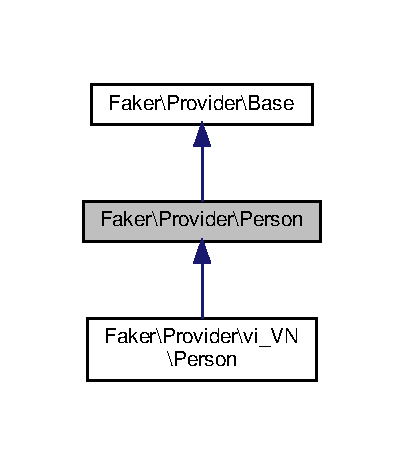
\includegraphics[width=194pt]{classFaker_1_1Provider_1_1Person__inherit__graph}
\end{center}
\end{figure}


Collaboration diagram for Faker\textbackslash{}Provider\textbackslash{}Person\+:\nopagebreak
\begin{figure}[H]
\begin{center}
\leavevmode
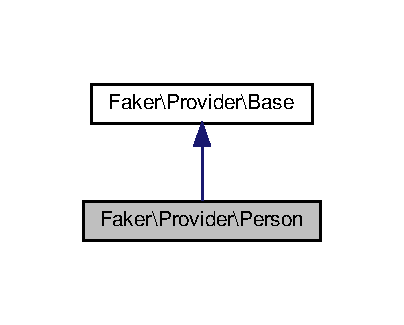
\includegraphics[width=194pt]{classFaker_1_1Provider_1_1Person__coll__graph}
\end{center}
\end{figure}
\subsection*{Public Member Functions}
\begin{DoxyCompactItemize}
\item 
\mbox{\Hypertarget{classFaker_1_1Provider_1_1Person_a612eb0e4dda01db0c06e29cc9af534a8}\label{classFaker_1_1Provider_1_1Person_a612eb0e4dda01db0c06e29cc9af534a8}} 
{\bfseries name} (\$gender=null)
\item 
\mbox{\Hypertarget{classFaker_1_1Provider_1_1Person_a63608efceaa9fa6a71d31cceb6385538}\label{classFaker_1_1Provider_1_1Person_a63608efceaa9fa6a71d31cceb6385538}} 
{\bfseries first\+Name} (\$gender=null)
\item 
\mbox{\Hypertarget{classFaker_1_1Provider_1_1Person_adf509b4ba24aba151b2dbb4e3dd982c6}\label{classFaker_1_1Provider_1_1Person_adf509b4ba24aba151b2dbb4e3dd982c6}} 
{\bfseries last\+Name} ()
\item 
\mbox{\Hypertarget{classFaker_1_1Provider_1_1Person_a2446c8e35d9ffb97008ba087a89f1b9e}\label{classFaker_1_1Provider_1_1Person_a2446c8e35d9ffb97008ba087a89f1b9e}} 
{\bfseries title} (\$gender=null)
\end{DoxyCompactItemize}
\subsection*{Static Public Member Functions}
\begin{DoxyCompactItemize}
\item 
\mbox{\Hypertarget{classFaker_1_1Provider_1_1Person_acc7056a4bfe1e64e8323384aaa721d27}\label{classFaker_1_1Provider_1_1Person_acc7056a4bfe1e64e8323384aaa721d27}} 
static {\bfseries first\+Name\+Male} ()
\item 
\mbox{\Hypertarget{classFaker_1_1Provider_1_1Person_a748194a63b272afda544b06dfba297c8}\label{classFaker_1_1Provider_1_1Person_a748194a63b272afda544b06dfba297c8}} 
static {\bfseries first\+Name\+Female} ()
\item 
\mbox{\Hypertarget{classFaker_1_1Provider_1_1Person_ae175cf00a252276dd39e6c34996b5f9d}\label{classFaker_1_1Provider_1_1Person_ae175cf00a252276dd39e6c34996b5f9d}} 
static {\bfseries title\+Male} ()
\item 
\mbox{\Hypertarget{classFaker_1_1Provider_1_1Person_afb11d111d5202224841c38051d0c5857}\label{classFaker_1_1Provider_1_1Person_afb11d111d5202224841c38051d0c5857}} 
static {\bfseries title\+Female} ()
\end{DoxyCompactItemize}
\subsection*{Public Attributes}
\begin{DoxyCompactItemize}
\item 
\mbox{\Hypertarget{classFaker_1_1Provider_1_1Person_a6b8dd195e7167f9eab92a04290271933}\label{classFaker_1_1Provider_1_1Person_a6b8dd195e7167f9eab92a04290271933}} 
const {\bfseries G\+E\+N\+D\+E\+R\+\_\+\+M\+A\+LE} = \textquotesingle{}male\textquotesingle{}
\item 
\mbox{\Hypertarget{classFaker_1_1Provider_1_1Person_a60a8d39672759d0b961a7df1f6b89a3a}\label{classFaker_1_1Provider_1_1Person_a60a8d39672759d0b961a7df1f6b89a3a}} 
const {\bfseries G\+E\+N\+D\+E\+R\+\_\+\+F\+E\+M\+A\+LE} = \textquotesingle{}female\textquotesingle{}
\end{DoxyCompactItemize}
\subsection*{Static Protected Attributes}
\begin{DoxyCompactItemize}
\item 
static {\bfseries \$title\+Format}
\item 
static {\bfseries \$first\+Name\+Format}
\item 
static {\bfseries \$male\+Name\+Formats}
\item 
static {\bfseries \$female\+Name\+Formats}
\end{DoxyCompactItemize}
\subsection*{Additional Inherited Members}


\subsection{Member Data Documentation}
\mbox{\Hypertarget{classFaker_1_1Provider_1_1Person_a1d9d04d0d19d759f1d33ef9c2502538c}\label{classFaker_1_1Provider_1_1Person_a1d9d04d0d19d759f1d33ef9c2502538c}} 
\index{Faker\+::\+Provider\+::\+Person@{Faker\+::\+Provider\+::\+Person}!\$female\+Name\+Formats@{\$female\+Name\+Formats}}
\index{\$female\+Name\+Formats@{\$female\+Name\+Formats}!Faker\+::\+Provider\+::\+Person@{Faker\+::\+Provider\+::\+Person}}
\subsubsection{\texorpdfstring{\$female\+Name\+Formats}{$femaleNameFormats}}
{\footnotesize\ttfamily Faker\textbackslash{}\+Provider\textbackslash{}\+Person\+::\$female\+Name\+Formats\hspace{0.3cm}{\ttfamily [static]}, {\ttfamily [protected]}}

{\bfseries Initial value\+:}
\begin{DoxyCode}
= array(
        \textcolor{stringliteral}{'\{\{firstNameFemale\}\} \{\{lastName\}\}'},
    )
\end{DoxyCode}
\mbox{\Hypertarget{classFaker_1_1Provider_1_1Person_a0d7cd0cc005038a274441a545f34e0b7}\label{classFaker_1_1Provider_1_1Person_a0d7cd0cc005038a274441a545f34e0b7}} 
\index{Faker\+::\+Provider\+::\+Person@{Faker\+::\+Provider\+::\+Person}!\$first\+Name\+Format@{\$first\+Name\+Format}}
\index{\$first\+Name\+Format@{\$first\+Name\+Format}!Faker\+::\+Provider\+::\+Person@{Faker\+::\+Provider\+::\+Person}}
\subsubsection{\texorpdfstring{\$first\+Name\+Format}{$firstNameFormat}}
{\footnotesize\ttfamily Faker\textbackslash{}\+Provider\textbackslash{}\+Person\+::\$first\+Name\+Format\hspace{0.3cm}{\ttfamily [static]}, {\ttfamily [protected]}}

{\bfseries Initial value\+:}
\begin{DoxyCode}
= array(
      \textcolor{stringliteral}{'\{\{firstNameMale\}\}'},
      \textcolor{stringliteral}{'\{\{firstNameFemale\}\}'},
    )
\end{DoxyCode}
\mbox{\Hypertarget{classFaker_1_1Provider_1_1Person_a5f99497ac66ab711fcafa342e4c5e97a}\label{classFaker_1_1Provider_1_1Person_a5f99497ac66ab711fcafa342e4c5e97a}} 
\index{Faker\+::\+Provider\+::\+Person@{Faker\+::\+Provider\+::\+Person}!\$male\+Name\+Formats@{\$male\+Name\+Formats}}
\index{\$male\+Name\+Formats@{\$male\+Name\+Formats}!Faker\+::\+Provider\+::\+Person@{Faker\+::\+Provider\+::\+Person}}
\subsubsection{\texorpdfstring{\$male\+Name\+Formats}{$maleNameFormats}}
{\footnotesize\ttfamily Faker\textbackslash{}\+Provider\textbackslash{}\+Person\+::\$male\+Name\+Formats\hspace{0.3cm}{\ttfamily [static]}, {\ttfamily [protected]}}

{\bfseries Initial value\+:}
\begin{DoxyCode}
= array(
        \textcolor{stringliteral}{'\{\{firstNameMale\}\} \{\{lastName\}\}'},
    )
\end{DoxyCode}
\mbox{\Hypertarget{classFaker_1_1Provider_1_1Person_a66e8dccc0b676a7147f6fdc7c9d03c4f}\label{classFaker_1_1Provider_1_1Person_a66e8dccc0b676a7147f6fdc7c9d03c4f}} 
\index{Faker\+::\+Provider\+::\+Person@{Faker\+::\+Provider\+::\+Person}!\$title\+Format@{\$title\+Format}}
\index{\$title\+Format@{\$title\+Format}!Faker\+::\+Provider\+::\+Person@{Faker\+::\+Provider\+::\+Person}}
\subsubsection{\texorpdfstring{\$title\+Format}{$titleFormat}}
{\footnotesize\ttfamily Faker\textbackslash{}\+Provider\textbackslash{}\+Person\+::\$title\+Format\hspace{0.3cm}{\ttfamily [static]}, {\ttfamily [protected]}}

{\bfseries Initial value\+:}
\begin{DoxyCode}
= array(
      \textcolor{stringliteral}{'\{\{titleMale\}\}'},
      \textcolor{stringliteral}{'\{\{titleFemale\}\}'},
    )
\end{DoxyCode}


The documentation for this class was generated from the following file\+:\begin{DoxyCompactItemize}
\item 
src/\+Faker/\+Provider/Person.\+php\end{DoxyCompactItemize}

%--- End generated contents ---

% Index
\backmatter
\newpage
\phantomsection
\clearemptydoublepage
\addcontentsline{toc}{chapter}{Index}
\printindex

\end{document}
